% Critical assignments (generated by figs_c3ch12.py).
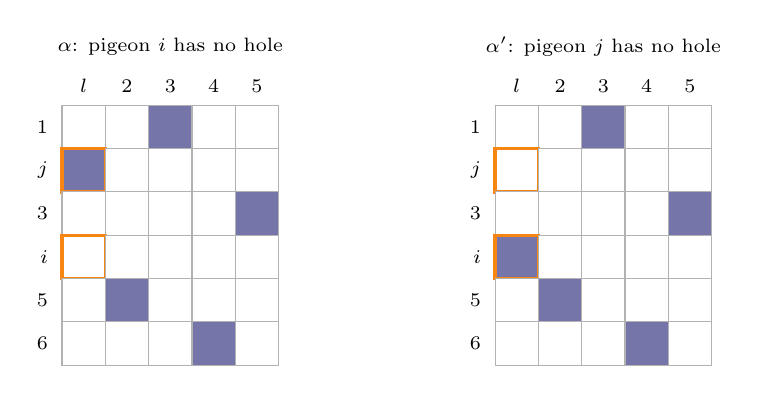
\begin{tikzpicture}[x=5.5mm,y=5.5mm,every node/.style={font=\scriptsize}]
\node[anchor=east] at (-0.1,-0.5) {$1$};
\draw[gray!60,fill=white] (0,0) rectangle (1,-1);
\draw[gray!60,fill=white] (1,0) rectangle (2,-1);
\draw[gray!60,fill=MidnightBlue!60] (2,0) rectangle (3,-1);
\draw[gray!60,fill=white] (3,0) rectangle (4,-1);
\draw[gray!60,fill=white] (4,0) rectangle (5,-1);
\node[anchor=east] at (-0.1,-1.5) {$j$};
\draw[BurntOrange,very thick,fill=MidnightBlue!60] (0,-1) rectangle (1,-2);
\draw[gray!60,fill=white] (1,-1) rectangle (2,-2);
\draw[gray!60,fill=white] (2,-1) rectangle (3,-2);
\draw[gray!60,fill=white] (3,-1) rectangle (4,-2);
\draw[gray!60,fill=white] (4,-1) rectangle (5,-2);
\node[anchor=east] at (-0.1,-2.5) {$3$};
\draw[gray!60,fill=white] (0,-2) rectangle (1,-3);
\draw[gray!60,fill=white] (1,-2) rectangle (2,-3);
\draw[gray!60,fill=white] (2,-2) rectangle (3,-3);
\draw[gray!60,fill=white] (3,-2) rectangle (4,-3);
\draw[gray!60,fill=MidnightBlue!60] (4,-2) rectangle (5,-3);
\node[anchor=east] at (-0.1,-3.5) {$i$};
\draw[BurntOrange,very thick,fill=white] (0,-3) rectangle (1,-4);
\draw[gray!60,fill=white] (1,-3) rectangle (2,-4);
\draw[gray!60,fill=white] (2,-3) rectangle (3,-4);
\draw[gray!60,fill=white] (3,-3) rectangle (4,-4);
\draw[gray!60,fill=white] (4,-3) rectangle (5,-4);
\node[anchor=east] at (-0.1,-4.5) {$5$};
\draw[gray!60,fill=white] (0,-4) rectangle (1,-5);
\draw[gray!60,fill=MidnightBlue!60] (1,-4) rectangle (2,-5);
\draw[gray!60,fill=white] (2,-4) rectangle (3,-5);
\draw[gray!60,fill=white] (3,-4) rectangle (4,-5);
\draw[gray!60,fill=white] (4,-4) rectangle (5,-5);
\node[anchor=east] at (-0.1,-5.5) {$6$};
\draw[gray!60,fill=white] (0,-5) rectangle (1,-6);
\draw[gray!60,fill=white] (1,-5) rectangle (2,-6);
\draw[gray!60,fill=white] (2,-5) rectangle (3,-6);
\draw[gray!60,fill=MidnightBlue!60] (3,-5) rectangle (4,-6);
\draw[gray!60,fill=white] (4,-5) rectangle (5,-6);
\node at (0.5,0.45) {$l$};
\node at (1.5,0.45) {$2$};
\node at (2.5,0.45) {$3$};
\node at (3.5,0.45) {$4$};
\node at (4.5,0.45) {$5$};
\node at (2.5,1.35) {$\alpha$: pigeon $i$ has no hole};
\node[anchor=east] at (9.9,-0.5) {$1$};
\draw[gray!60,fill=white] (10,0) rectangle (11,-1);
\draw[gray!60,fill=white] (11,0) rectangle (12,-1);
\draw[gray!60,fill=MidnightBlue!60] (12,0) rectangle (13,-1);
\draw[gray!60,fill=white] (13,0) rectangle (14,-1);
\draw[gray!60,fill=white] (14,0) rectangle (15,-1);
\node[anchor=east] at (9.9,-1.5) {$j$};
\draw[BurntOrange,very thick,fill=white] (10,-1) rectangle (11,-2);
\draw[gray!60,fill=white] (11,-1) rectangle (12,-2);
\draw[gray!60,fill=white] (12,-1) rectangle (13,-2);
\draw[gray!60,fill=white] (13,-1) rectangle (14,-2);
\draw[gray!60,fill=white] (14,-1) rectangle (15,-2);
\node[anchor=east] at (9.9,-2.5) {$3$};
\draw[gray!60,fill=white] (10,-2) rectangle (11,-3);
\draw[gray!60,fill=white] (11,-2) rectangle (12,-3);
\draw[gray!60,fill=white] (12,-2) rectangle (13,-3);
\draw[gray!60,fill=white] (13,-2) rectangle (14,-3);
\draw[gray!60,fill=MidnightBlue!60] (14,-2) rectangle (15,-3);
\node[anchor=east] at (9.9,-3.5) {$i$};
\draw[BurntOrange,very thick,fill=MidnightBlue!60] (10,-3) rectangle (11,-4);
\draw[gray!60,fill=white] (11,-3) rectangle (12,-4);
\draw[gray!60,fill=white] (12,-3) rectangle (13,-4);
\draw[gray!60,fill=white] (13,-3) rectangle (14,-4);
\draw[gray!60,fill=white] (14,-3) rectangle (15,-4);
\node[anchor=east] at (9.9,-4.5) {$5$};
\draw[gray!60,fill=white] (10,-4) rectangle (11,-5);
\draw[gray!60,fill=MidnightBlue!60] (11,-4) rectangle (12,-5);
\draw[gray!60,fill=white] (12,-4) rectangle (13,-5);
\draw[gray!60,fill=white] (13,-4) rectangle (14,-5);
\draw[gray!60,fill=white] (14,-4) rectangle (15,-5);
\node[anchor=east] at (9.9,-5.5) {$6$};
\draw[gray!60,fill=white] (10,-5) rectangle (11,-6);
\draw[gray!60,fill=white] (11,-5) rectangle (12,-6);
\draw[gray!60,fill=white] (12,-5) rectangle (13,-6);
\draw[gray!60,fill=MidnightBlue!60] (13,-5) rectangle (14,-6);
\draw[gray!60,fill=white] (14,-5) rectangle (15,-6);
\node at (10.5,0.45) {$l$};
\node at (11.5,0.45) {$2$};
\node at (12.5,0.45) {$3$};
\node at (13.5,0.45) {$4$};
\node at (14.5,0.45) {$5$};
\node at (12.5,1.35) {$\alpha'$: pigeon $j$ has no hole};
\end{tikzpicture}
